\documentclass[11pt, a4paper]{article}
\usepackage{pdfpages}
\usepackage{parallel}
\usepackage[T2A]{fontenc}
\usepackage{ucs}
\usepackage[utf8x]{inputenc}
\usepackage[polish,english,russian]{babel}
\usepackage{hyperref}
\usepackage{rotating}
\usepackage[inner=2cm,top=1.8cm,outer=2cm,bottom=2.3cm,nohead]{geometry}
\usepackage{listings}
\usepackage{graphicx}
\usepackage{wrapfig}
\usepackage{longtable}
\usepackage{indentfirst}
\usepackage{array}
\usepackage{tikzsymbols}
\usepackage{soul}
\usepackage[ruled,vlined]{algorithm2e}
%\counterwithout{figure}{section} 

\usepackage{url}
\makeatletter
\g@addto@macro{\UrlBreaks}{\UrlOrds}
\makeatother

\newcolumntype{P}[1]{>{\raggedright\arraybackslash}p{#1}}
\frenchspacing
\usepackage{fixltx2e} %text sub- and superscripts
\usepackage{icomma} % коскі ў матэматычным рэжыме
\PreloadUnicodePage{4}

\newcommand{\longpage}{\enlargethispage{\baselineskip}}
\newcommand{\shortpage}{\enlargethispage{-\baselineskip}}

\def\switchlang#1{\expandafter\csname switchlang#1\endcsname}
\def\switchlangbe{
\let\saverefname=\refname%
\def\refname{Літаратура}%
\def\figurename{Іл.}%
}
\def\switchlangen{
\let\saverefname=\refname%
\def\refname{References}%
\def\figurename{Fig.}%
}
\def\switchlangru{
\let\saverefname=\refname%
\let\savefigurename=\figurename%
\def\refname{Литература}%
\def\figurename{Рис.}%
}

\hyphenation{admi-ni-stra-tive}
\hyphenation{ex-pe-ri-ence}
\hyphenation{fle-xi-bi-li-ty}
\hyphenation{Py-thon}
\hyphenation{ma-the-ma-ti-cal}
\hyphenation{re-ported}
\hyphenation{imp-le-menta-tions}
\hyphenation{pro-vides}
\hyphenation{en-gi-neering}
\hyphenation{com-pa-ti-bi-li-ty}
\hyphenation{im-pos-sible}
\hyphenation{desk-top}
\hyphenation{elec-tro-nic}
\hyphenation{com-pa-ny}
\hyphenation{de-ve-lop-ment}
\hyphenation{de-ve-loping}
\hyphenation{de-ve-lop}
\hyphenation{da-ta-ba-se}
\hyphenation{plat-forms}
\hyphenation{or-ga-ni-za-tion}
\hyphenation{pro-gramming}
\hyphenation{in-stru-ments}
\hyphenation{Li-nux}
\hyphenation{sour-ce}
\hyphenation{en-vi-ron-ment}
\hyphenation{Te-le-pathy}
\hyphenation{Li-nux-ov-ka}
\hyphenation{Open-BSD}
\hyphenation{Free-BSD}
\hyphenation{men-ti-on-ed}
\hyphenation{app-li-ca-tion}

\def\progref!#1!{\texttt{#1}}
\renewcommand{\arraystretch}{2} %Іначай формулы ў матрыцы зліпаюцца з лініямі
\usepackage{array}

\def\interview #1 (#2), #3, #4, #5\par{

\section[#1, #3, #4]{#1 -- #3, #4}
\def\qname{LVEE}
\def\aname{#1}
\def\q ##1\par{{\noindent \bf \qname: ##1 }\par}
\def\a{{\noindent \bf \aname: } \def\qname{L}\def\aname{#2}}
}

\def\interview* #1 (#2), #3, #4, #5\par{

\section*{#1\\{\small\rm #3, #4. #5}}
\ifx\ParallelWhichBox\undefined%
    \addcontentsline{toc}{section}{#1, #3, #4}%
\else%
\ifnum\ParallelWhichBox=0%
    \addcontentsline{toc}{section}{#1, #3, #4}%
\fi\fi%

\def\qname{LVEE}
\def\aname{#1}
\def\q ##1\par{{\noindent \bf \qname: ##1 }\par}
\def\a{{\noindent \bf \aname: } \def\qname{L}\def\aname{#2}}
}

\newcommand{\interviewfooter}[1]{
\vskip 1em
\noindent \textit{#1}
}

\switchlang{ru}
\begin{document}

\title{2000 "--- Loas/Celltrix Ball Less Mouse}
\date{}
\maketitle
\selectlanguage{russian}

Мышь Ball Less Mouse, фигурирующая также под номером модели MUS-P241SL (рис. \ref{fig:BallLessMousePic}), была представлена на японском рынке в 2000 году. Компаниея Loas специализировалась на производстве и продаже компьютерной мебели, расходных материалов и других товаров, связанных с компьютерной техникой \cite{loas}. При этом, будучи интегратором, она активно предлагала под своим брэндом товары других производителей. В частности, разработка и выпуск MUS-P241SL были осуществлены тайваньской компанией Celltrix Technology, наиболее известной благодаря своему устройству Celtrix Trackbar (альтернативному средству управления курсором на основе вращающегося цилиндра). Конструкция Ball Less Mouse является не менее необычной: по всей видимости, это была последняя в истории компьютерная мышь на основе патента Xerox 1973 года, описывающего регистрацию движения на основе двух ортогональных колес \cite{pat}.

\begin{figure}[h]
    \centering
    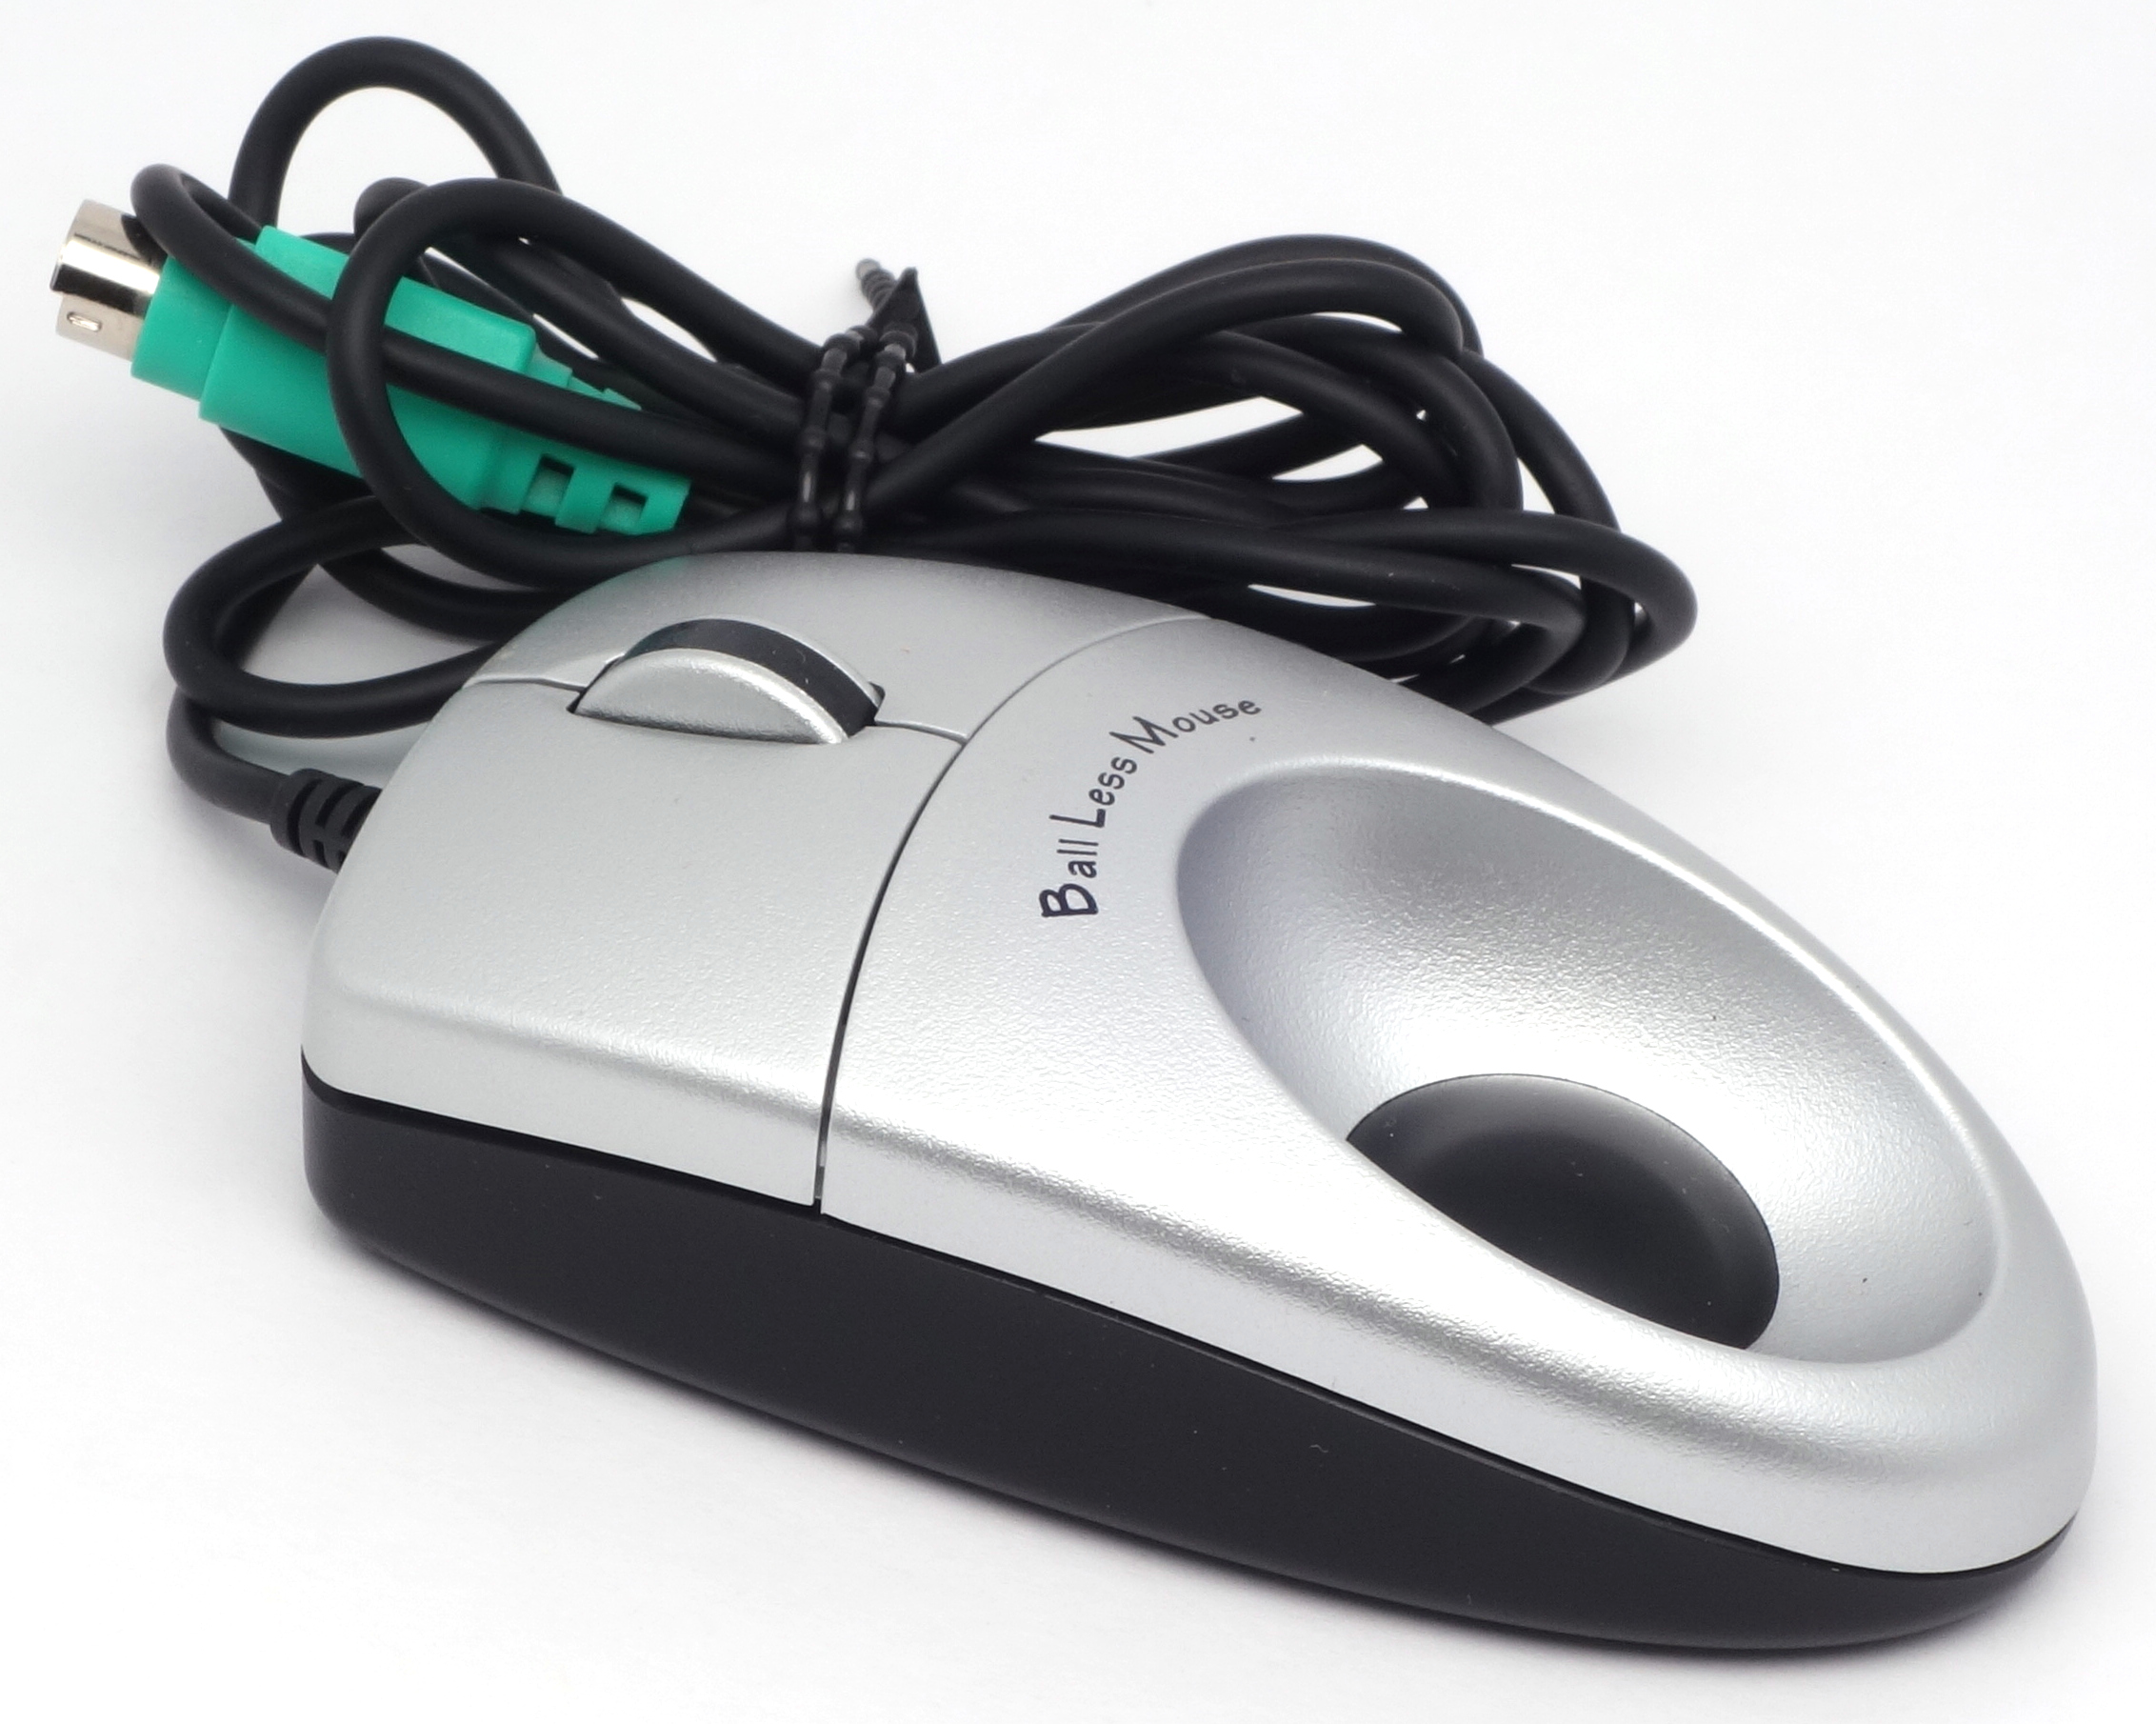
\includegraphics[scale=0.6]{2000_loas_ball_less_mouse/pic_30.jpg}
    \caption{Ball Less Mouse}
    \label{fig:BallLessMousePic}
\end{figure}

Согласно информации на сайте Loas, мышь была доступна в трех версиях: MUS-P241BK (черная), MUS-P241SL (серебристая) и MUS-P241VA (фиолетово-серая) \cite{details}. В качестве уникальных технических особенностей устройства производитель выделял «механизм прямого привода» и «плавную, бесступенчатую прокрутку». На упаковке также подчеркивается использование двух роликов вместо шара, благодаря чему мышь избавлена от необходимости в чистке и/или использовании коврика \cite{package}.

\section*{Внешний вид}

Корпус мыши MUS-P241SL выполнен в серебристо-черной цветовой гамме и имеет клиновидный силуэт, достаточно типичный для мышей 2000-х годов: он расширяется в области кнопок, чтобы обеспечить им максимальную площадь, и плавно сужается к области запястья. Верхняя часть корпуса "--- серебристая, и ее ближнюю к пользователю половину занимает декоративная зона, креативно обыгрывающая отсутствие шара. На виде сверху она визуально напоминает разрезанный плод авокадо, но по факту это полость, образованная формой вытянутого сфероида, на дне которой находится выпуклый сегмент сферы черного цвета, символизирующий тот самый шар, которого у мыши нет (рис. \ref{fig:BallLessMouseTopBottom}). В центральной части, между этой декоративной полостью и зоной кнопок, находится изогнутая грамматически спорная надпись <<Ball Less Mouse>>. Кроме того, на виде сверху можно заметить ребристую муфту, защищающую кабель, две кнопки, вписанные в форму корпуса, и находящееся между ними крупное колесо прокрутки. Колесо прокрутки подпружинено и при нажатии слегка утапливается, однако в отличие от других мышей, не выполняет функцию третьей кнопки.

\begin{figure}[h]
    \centering
    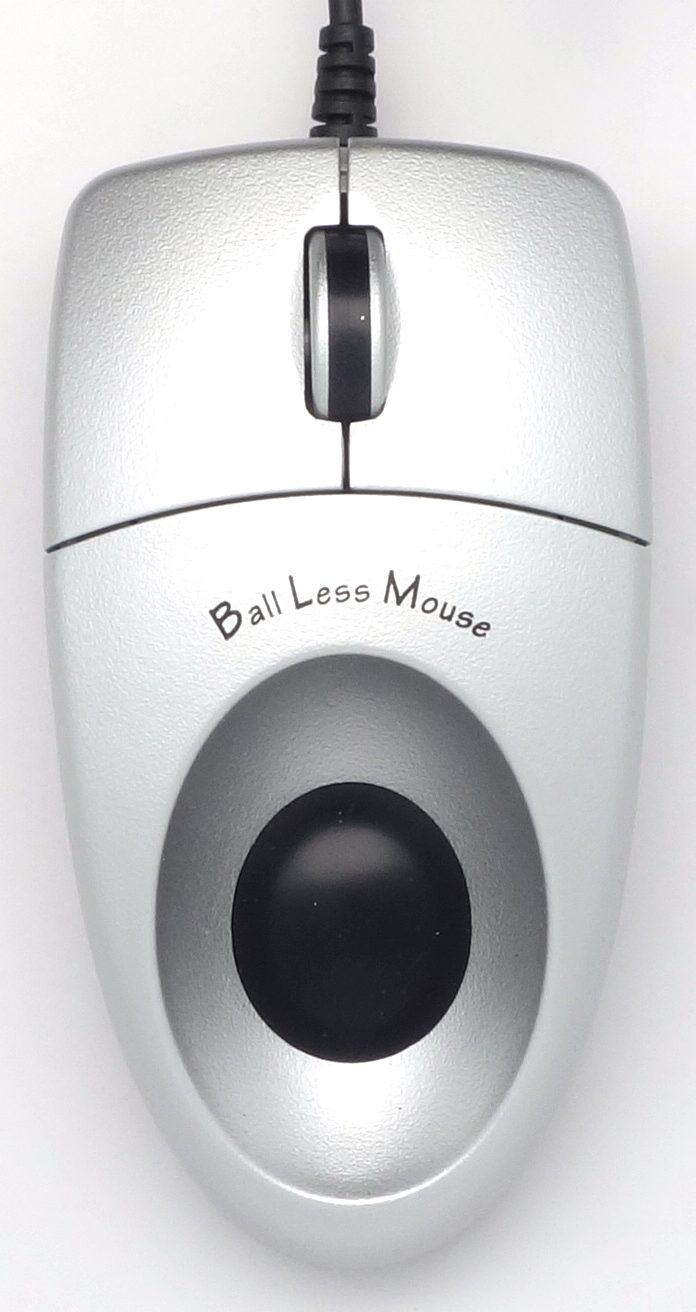
\includegraphics[scale=0.6]{2000_loas_ball_less_mouse/top_30.jpg}
    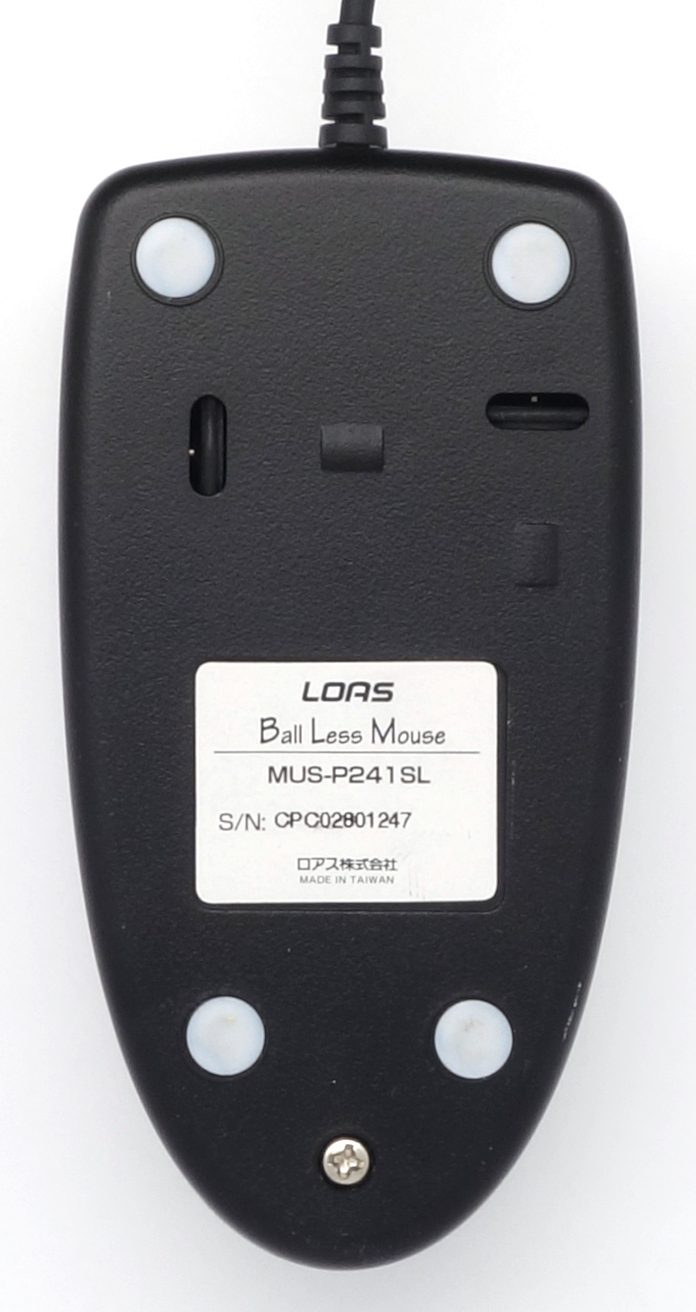
\includegraphics[scale=0.6]{2000_loas_ball_less_mouse/bottom_15.jpg}
    \caption{Ball Less Mouse вид сверху и снизу}
    \label{fig:BallLessMouseTopBottom}
\end{figure}

Нижняя часть корпуса "--- черного цвета. Она содержит наклейку с информационными данными, круглые накладки из низкофрикционного материала, облегчающие скольжение мыши, а также две прорези, из которых выступают колеса, предназначенные для регистрации движения. Колеса расположены ортогонально друг другу, чтобы при продольном и поперечном движении одно из них вращалось, а другое проскальзывало, а их оси расположены под углом к горизонтальной плоскости для лучшей регистрации диагональных перемещений.

\section*{Размеры и эргономика}

Помимо упомянутых особенностей, Ball Less Mouse представляет собой устройство, имеющее типичные для 2000-х годов размеры и форму (рис. \ref{fig:BallLessMouseSize}). Мышь имеет симметричный корпус и одинаково удобна для управления левой и правой рукой.

\begin{figure}[h]
    \centering
    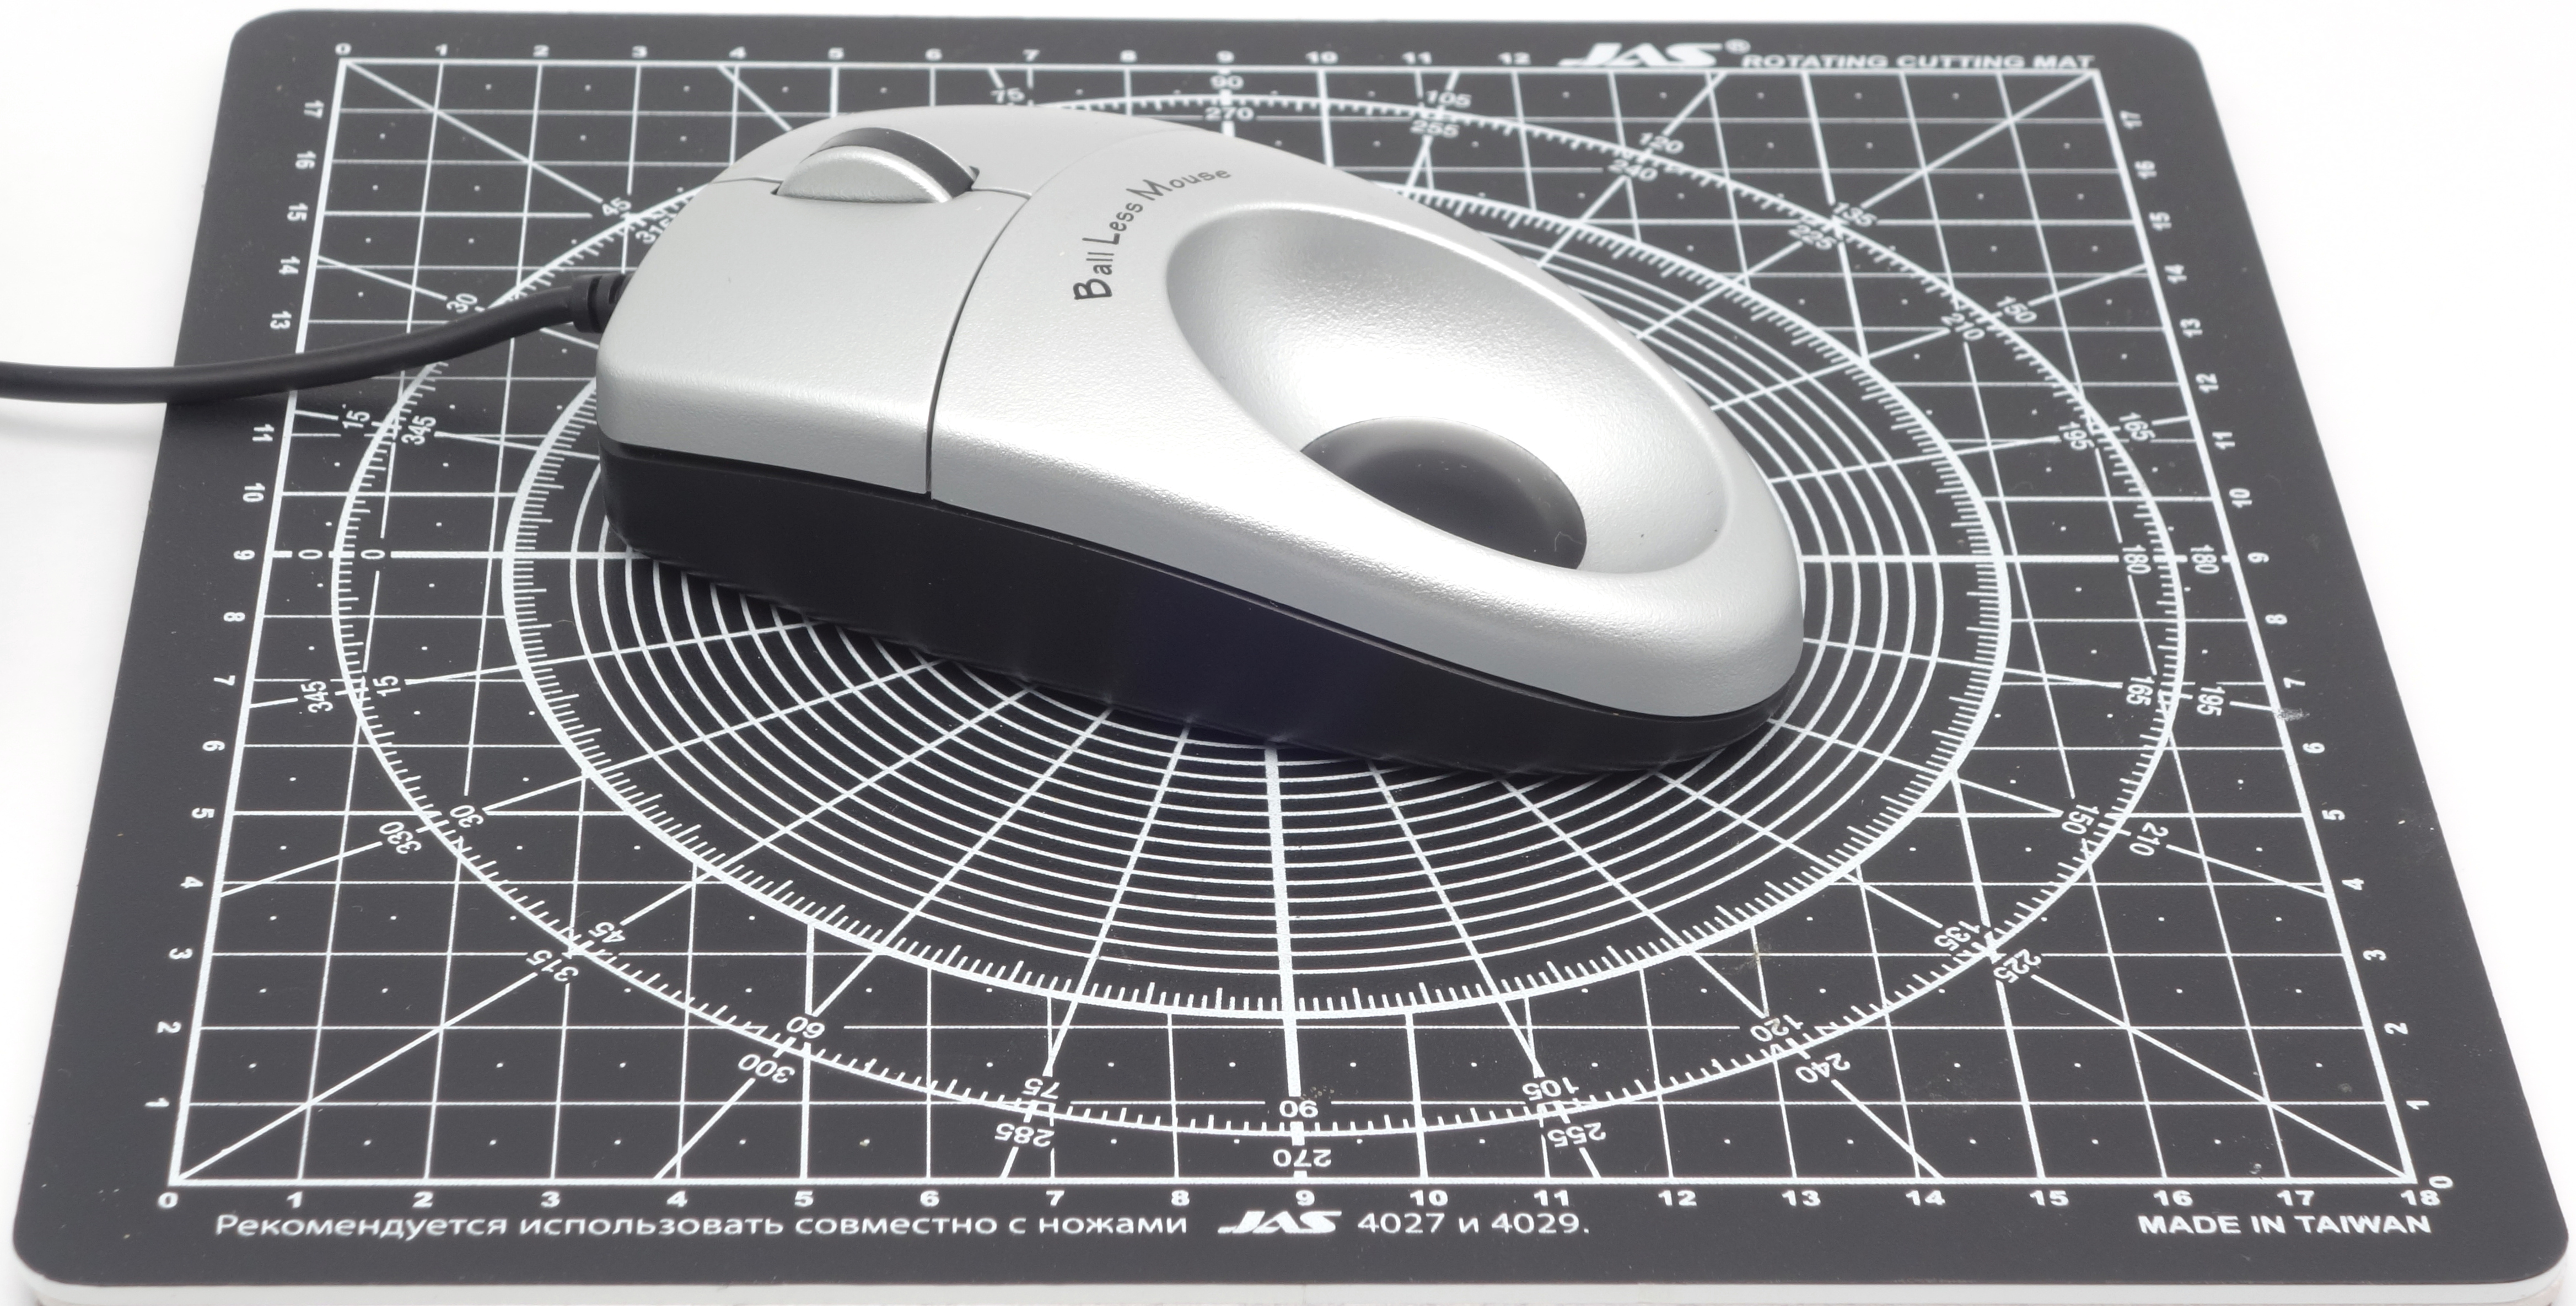
\includegraphics[scale=0.3]{2000_loas_ball_less_mouse/size_15.jpg}
    \caption{Ball Less Mouse на размерном коврике с шагом сетки 1~см}
    \label{fig:BallLessMouseSize}
\end{figure}

Форма корпуса и кнопок, отвечающая стандартам 2000-х годов, обеспечивает удобное положение ладони (рис. \ref{fig:BallLessMouseHand}). Встроенная в корпус полость с <<имитатором шара>> меньше ладони пользователя, полностью накрывается ею и не оказывает существенного влияния на удобство пользования мышью. Однако этого нельзя сказать об использовании колеса прокрутки: руководство пользователя аккуратно уточняет, что пользователь может <<прокручивать экран вверх и вниз, нажимая и вращая колесо>>, и лишний раз подчеркивает, что для прокрутки экрана необходимо <<нажав и удерживая колесо, повернуть его>> \cite{manual}. Это делает скроллинг существенно более трудоемким процессом, поскольку задействует дополнительное мускульное усилие (ситуация аналогична удерживанию нажатой кнопки при перетаскивании). Очевидно, что такой механизм скроллинга при активном и длительном использовании прокрутки должен вызывать утомляемость и болезненные ощущения в задействованных мышцах.

В руководстве пользователя также отмечается, что не поддерживается панорамная прокрутка путем перетаскивания мыши с нажатой третьей кнопкой, однако это очевидное следствие того, что мышь является двухкнопочной.

\begin{figure}[h]
    \centering
    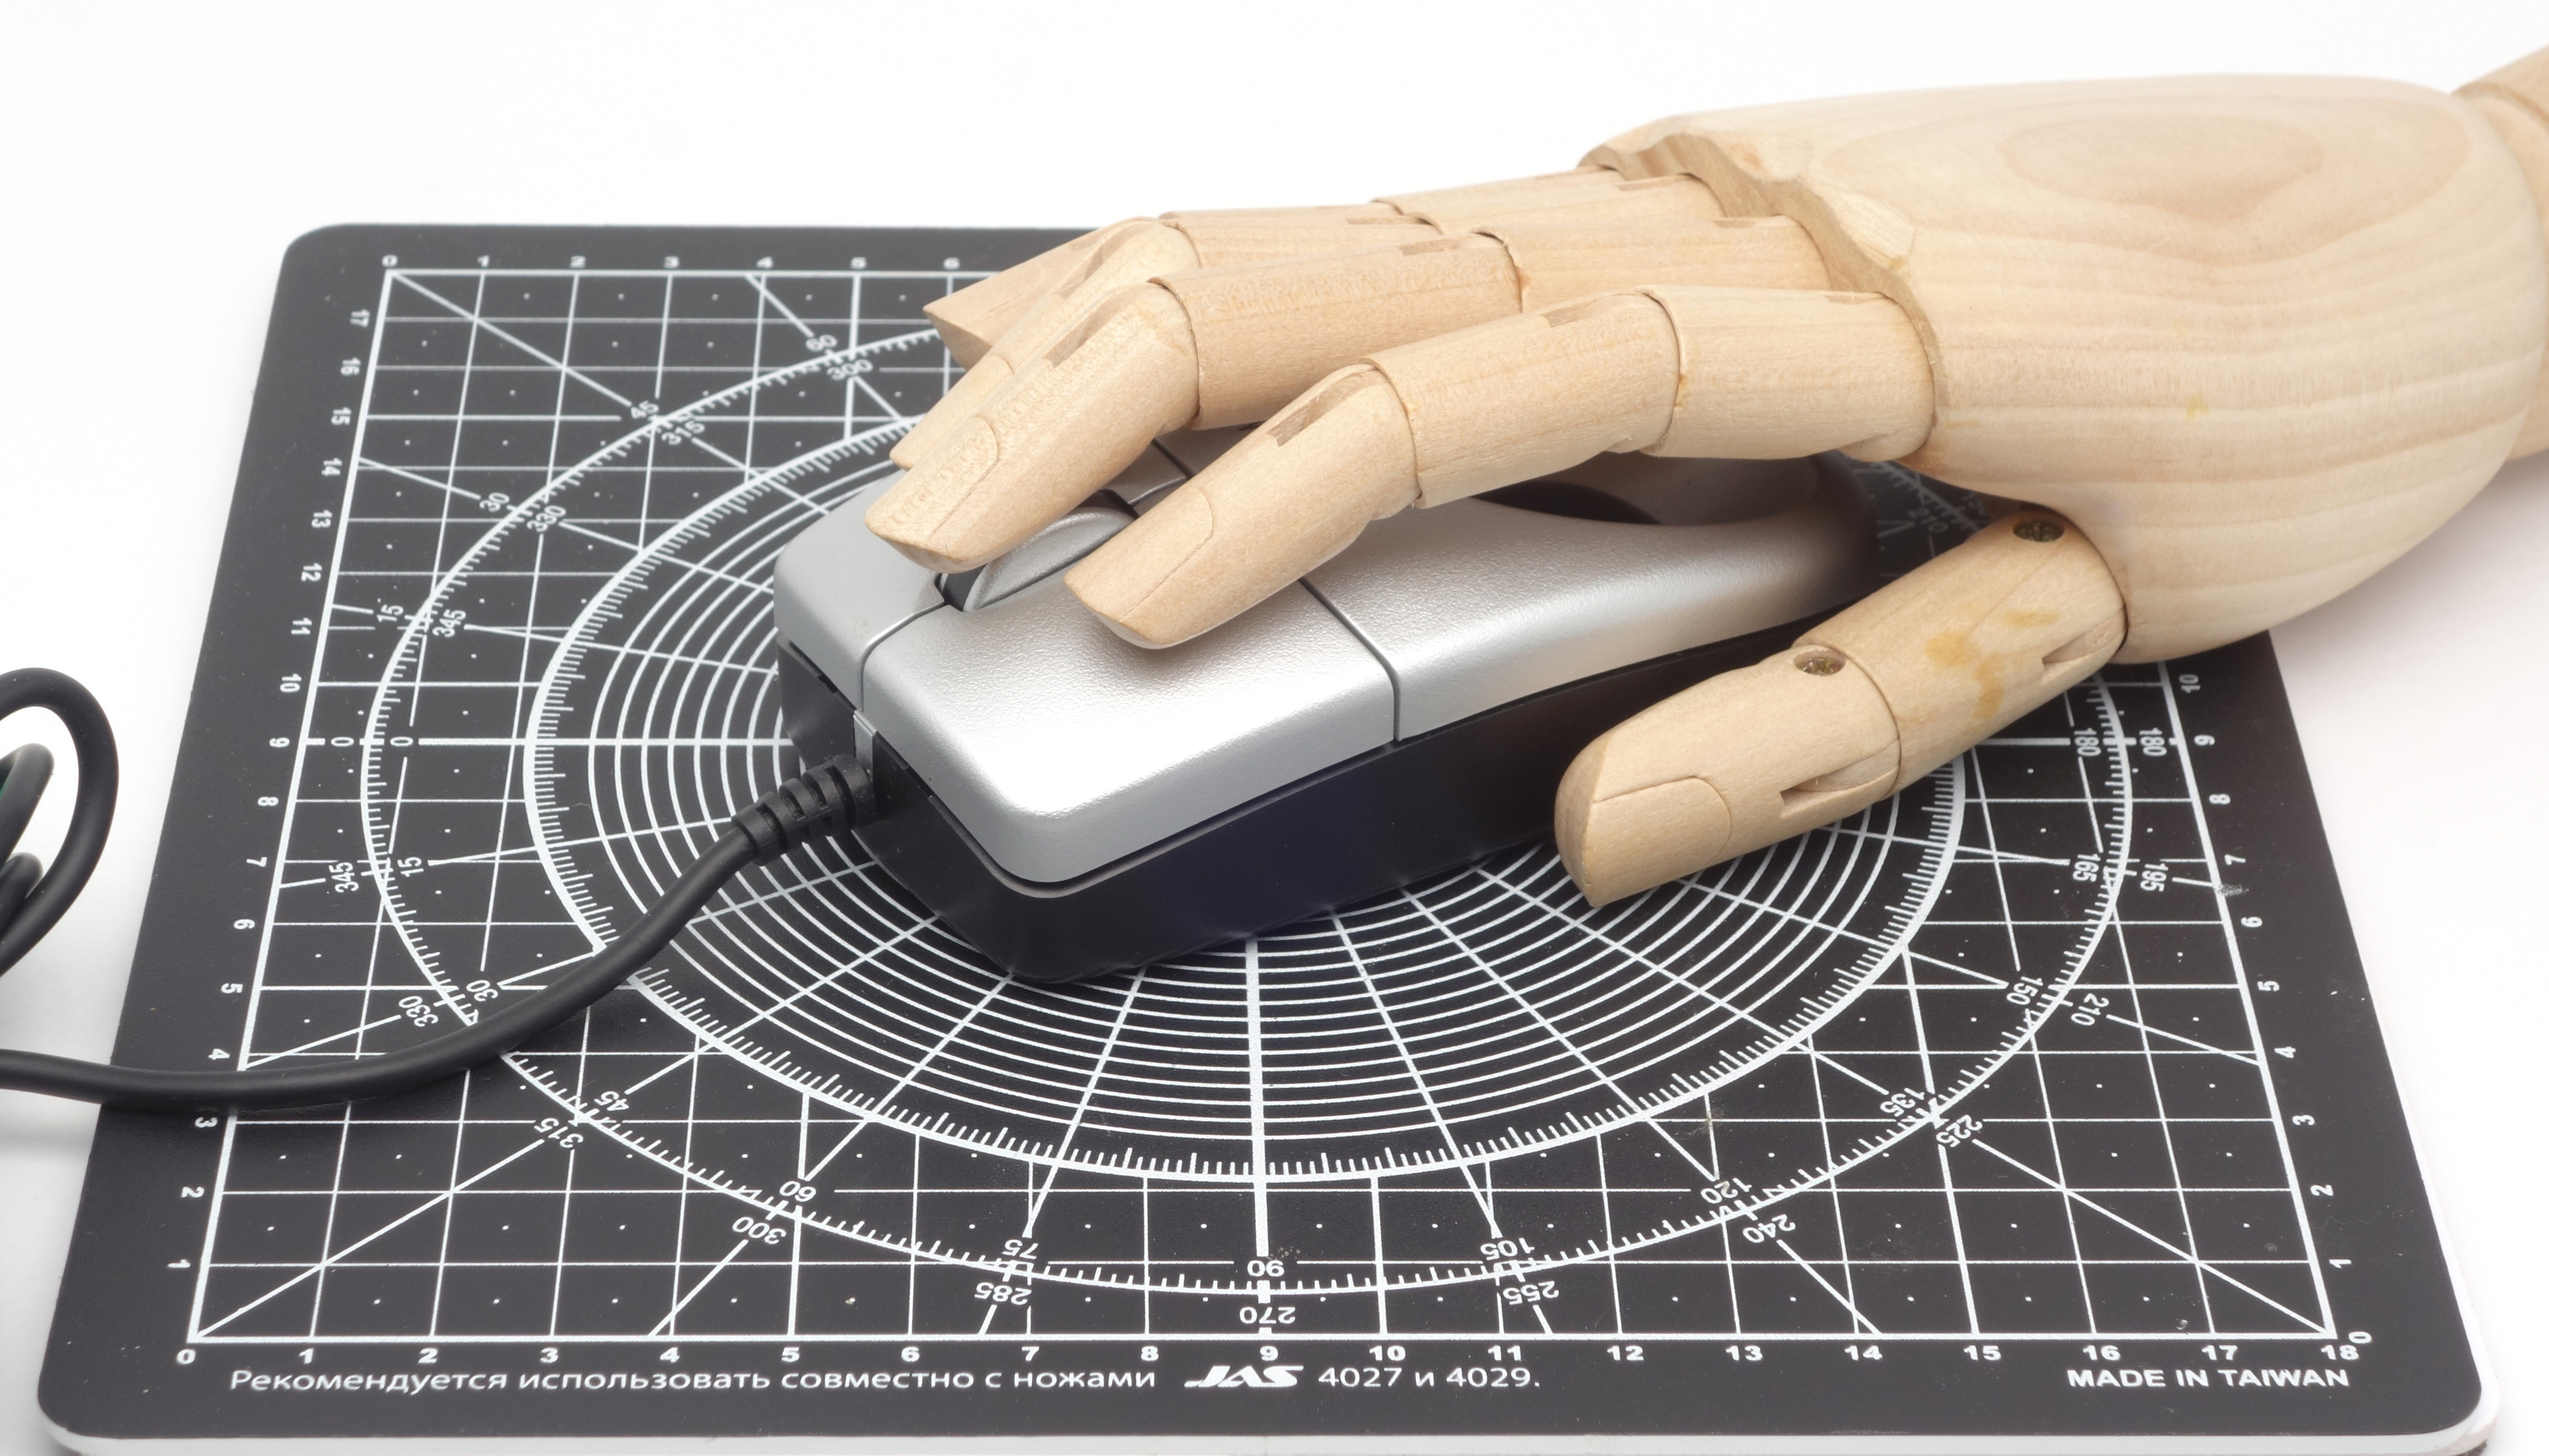
\includegraphics[scale=0.3]{2000_loas_ball_less_mouse/hand_15.jpg}
    \caption{Изображение Ball Less Mouse с моделью руки человека}
    \label{fig:BallLessMouseHand}
\end{figure}

\section*{Подключение}

Согласно описанию на сайте компании \cite{details}, мышь MUS-P241 выпускалась исключительно с интерфейсом PS/2, и предназначалась для использования с компьютерами на базе архитектуры x86 "--- в частности, DOS/V-совместимыми компьютерами и Windows-совместимыми NEC PC98-NX. Производитель не комплектовал мышь какими-либо драйверами или другим программным обеспечением, полностью полагаясь на встроенные драйвера операционных систем, в числе которых были заявлены Windows 98 и Windows 2000, а также в ограниченном варианте, Windows 95 (ограничения этой ОС не позволяли использовать колесо прокрутки). 

\section*{Внутреннее устройство}

Внутреннее устройство мыши, показанное на рисунке \ref{fig:BallLessMouseInside}, позволяет классифицировать ее как оптомеханическую.
Конструкция оптических прерывателей крайне необычна: они имеют форму цилиндров с чередующимися продольными полосами из чернного и белого пластика (в отличие от традиционных оптических прерывателей, рабочей поверхностью которых является торец диска). 
Сдвоенный белый блок в центре печатной платы закрывает два фотоприемника и ортогональные друг другу световоды. Свет от каждого из двух светодиодов, расположенных снаружи блока, отражается от белых полос на оптических прерывателях, а затем по световодам попадает на фотоприемники. Очевидно, что использование простой белой пластмассы в качестве отражающей поверхности стало возможным благодаря чувствительности фотоприемников, заметно равзившейся по сравнению с 80-ми годами, для которых характерна конструкция классической мыши с колесами.

В механическом смысле мышь повторяет конструкцию своих аналогов, выпускавшихся в 1980-е годы: энкодеры закреплены непосредственно на осях колес. Это конструкция компании Torrington, реализованная в её механической мыши Manager Mouse и ее модификациях: TPX Mouse от Tropic Informática и оптической Manager Mouse от Numonics. Очевидно, это и есть «механизм прямого привода», упоминаемый в описании Ball Less Mouse \cite{details}.

Что касается второй особенности "--- «плавной, бесступенчатой прокрутки» "--- она объясняется тем, что мышь имеет всего два энкодера, и один и тот же энкодер используется при скроллинге и при вертикальном перемещении курсора. Для механического разделения колеса прокрутки и колеса продольного перемещения мыши использован подвес энкодера на пружинах. При нажатии на колесо прокрутки оно опускается и получает механический контакт с энкодером; одновременно с этим пружина подтягивает вверх ось колеса, отвечающего за вертикальное перемещение курсора, чтобы оно могло свободно вращаться, не касаясь рабочей поверхности стола. Роль кнопок, отключающих передачу вертикальных координат при скроллинге, видимо играют пружины, замыкающие электрический контакт при нажатии на колесо прокрутки.

Безусловно, такая конструкция не позволяет пользователю перемещать курсор по вертикали одновременно с прокруткой, но эта задача нетипична и едва ли востребована. Взамен она обеспечивает максимально плавную прокрутку и позволяет выполнять ее с очень высокой точностью и высоким разрешением (что также не требуется для типичных пользовательских задач). А вот необходимость надавливать на колесо прокрутки для скроллинга остается действительно существенным недостатком конструкции.

Разрешение мыши существенно повышено по сравнению с ее колесными прототипами 1980-х годов (этому способствуют использование более современного микроконтроллера и оптомеханическая часть с бóльшими колесами): по информации на упаковке оно составляет 625 DPI \cite{package}.


\begin{figure}[h]
    \centering
    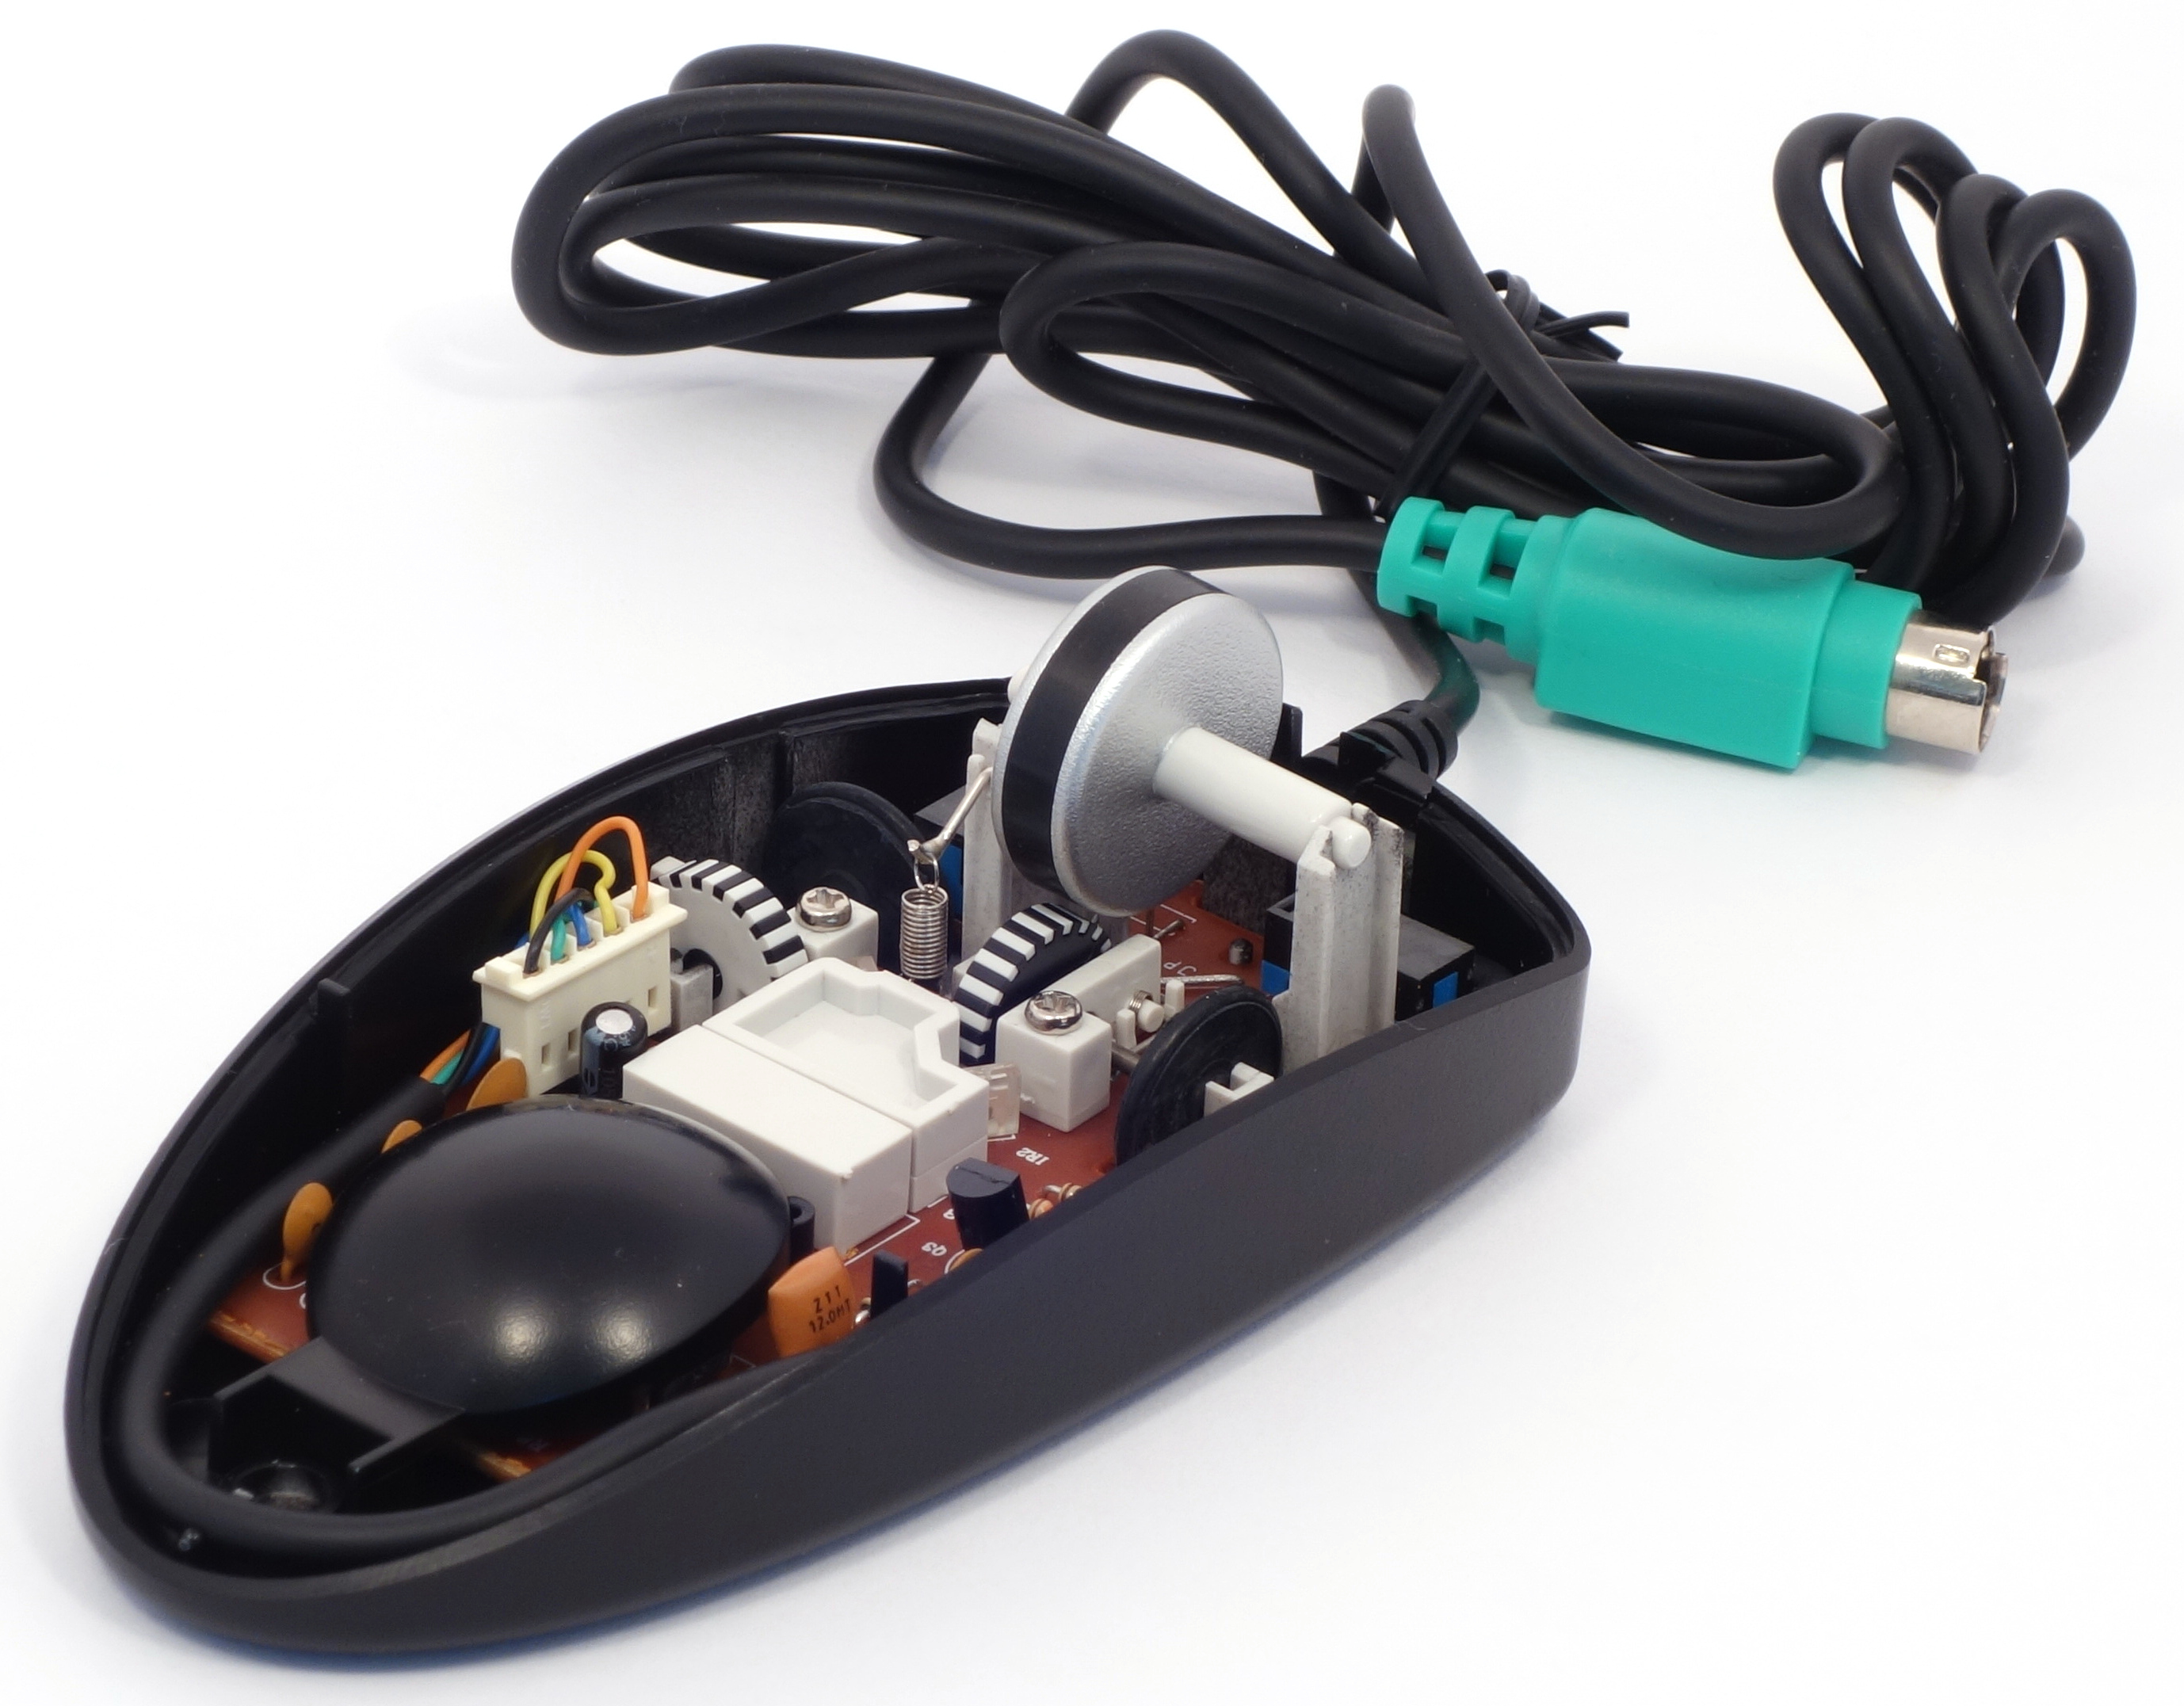
\includegraphics[scale=0.8]{2000_loas_ball_less_mouse/inside_30.jpg}
    \caption{Ball Less Mouse в разобранном виде}
    \label{fig:BallLessMouseInside}
\end{figure}

В числе надписей на печатной плате присутствуют строки <<CELLTRIX MOUSE V2000315>> и <<Feb 19 Y2K>>, что позволяет определить производителя мыши, а также, вместе с упоминанием на сайте компании Loas \cite{catalog} позволяет датировать ее 2000 годом.

\begin{thebibliography}{9}
\bibitem{loas} Company profile -- loas.co.jp [in Japanese] \url{https://web.archive.org/web/20010413213735fw_/http://www.loas.co.jp/KA.html}
\bibitem{pat} Transducer for a display-oriented pointing device \url{https://patents.google.com/patent/US3892963A/en}
\bibitem{details} Ball-less mouse -- loas.co.jp [in Japanese] \url{https://web.archive.org/web/20010426185102/http://www.loas.co.jp/MUCA7.htm}
\bibitem{package} Ball-less mouse cardbox [in Japanese] \url{https://raw.githubusercontent.com/fiowro/mouses/main/source/OCR/loas_mouse_box.pdf}
\bibitem{manual} MUS-P241 Series Ball-less Mouse Instruction Manual [in Japanese] \url{https://raw.githubusercontent.com/fiowro/mouses/main/source/OCR/loas_mouse_manual.pdf}
\bibitem{catalog} Mouse Catalog -- loas.co.jp [in Japanese] \url{https://web.archive.org/web/20001027054116fw_/http://www.loas.co.jp/MUCA.htm}
\end{thebibliography}
\end{document}
